\chapter{Cryptographic primitives}
\label{chpr:crypto_primitives}
In this section we present the cryptographic primitives which are necessary to build a \textit{confidential transaction}.\\
Prior to this, however, we start with a crash dive into some pillars of Elliptic Curve Cryptography (ECC), the focus being just on what can be useful to follow the incoming narration. We refer to \cite{Sec} or \cite{UnderstandingCrypto} for a more deep approach.\\
Elliptic Curve Cryptography is a public-key cryptosystem built on elliptic curves defined over finite fields and, for our purposes, it is the cryptosystem Bitcoin uses to secure the transactions. It is based on the intractability of the Elliptic Curve Discrete Logarithm Problem (ECDLP), namely the infeasibility of computing the discrete logarithm of a random elliptic curve point with respect to a publicly known base point\footnote{At the base of public-key cryptography there is always the intractability of a particular mathematical problem: \begin{itemize} \item RSA public-key schemes: hardness of factoring large integers. \item DLP-based public-key schemes: hardness of solving the discrete logarithm problem. \item ECDLP-based public-key schemes: hardness of solving the generalized discrete logarithm over an elliptic curve. \end{itemize}}. The benefits over its prior alternatives (in the field of public-key or asymmetric cryptography) come from the possibility of providing the same security level with shorter operands, which is in turn a consequence of the problem being harder to solve. Indeed, it is even the latest solution which has come out among the mentioned alternatives.\\
Referring to the Appendix \ref{app:A} for both the definition of finite field (and how to get to it) and the presentation of the DLP (in its non-elliptic curve formulations) to avoid making this introduction unintentionally cumbersome, we give instead here the definition of \textit{elliptic curve} and we present the known translation of the DLP over elliptic curves (ECDLP).\\ 
The need to introduce elliptic curves is motivated by the necessity of searching a cyclic group where to build the cryptosystem\footnote{See DLP arguments in section \ref{DLP} for more details.}; observe, however, that the mere existence of a cyclic group is not sufficient, the problem being to find such one where the DLP is computationally hard to solve. It turns out that elliptic curves are fitted for the purpose and thus the goal becomes to find elliptic curves with a large cyclic group. Later in this section, a theorem will support the suitability of elliptic curves in providing such a result, thus explaining their fundamental role in the discussion.\\
As remarked within the Appendix \ref{app:A}, for cryptographic use, the focus is just on elliptic curves defined over a finite field (in particular we consider $K = \mathbb{F}_p$, the finite field with $p$ elements) rather than over generic fields (the set $\mathbb{R}$ being an example).
\begin{mydef}
\label{def_EC}
    The elliptic curve over $\mathbb{F}_p$\footnote{Which we denote by $E(\mathbb{F}_p)$.} is the set of all pairs $(x,y) \in \mathbb{F}_p$ such that $\{(x,y) \in \mathbb{F}_p \times \mathbb{F}_p: y^2 = x^3 + ax+b \mod p\} \cup \{\infty\}$ with $a,b \in \mathbb{F}_p$ and such that the consistency condition $4 a^3+27b^2 \neq 0 \mod{p}$ holds true.
\end{mydef}
\noindent
The problem now becomes both identifying the group elements and defining a group operation with these elements. Group elements are nothing else than the points fulfilling the curve equation in Definition \ref{def_EC}. The definition of the group operation is not presented here, for the details we refer to \cite{UnderstandingCrypto}.\\
The only point we want to stress is the meaning of $\{\infty \}$ in Definition \ref{def_EC}:
\begin{myrem}
    $\{\infty \}$ is the so called infinity point and turns out to be the identity element of the group defined by the points over the elliptic curve together with its group operation.
\end{myrem}
\noindent
At this point, it is possible to state the following theorem, which eventually closes the circle by explaining the reason why it is possible to build a DLP with elliptic curves.
\begin{mytheorem}
    The points on an elliptic curve, together with the infinity point $\{\infty \}$ (other than defining a group by themselves once the group operation is defined) have cyclic subgroups. Moreover, under certain conditions (merely if the group order is prime) all points on an elliptic curve form a cyclic group.
\end{mytheorem}
\begin{myrem}
    By specializing the notation seen in the Appendix \ref{app:A} to the elliptic curve case, we denote by $G$ the generator of a cyclic (sub)group defined over an elliptic curve (being an element of the (sub)group itself, it is nothing else than a point on the curve). Thus, starting from $G$ it is possible to explore the entire (sub)group (thus recovering all the (sub)group points) by repeatedly applying the group operation to $G$.
\end{myrem}
\begin{myrem}
    If the EC (sub)group has order $m$, the application of the EC group operation $m$ times gives back the identity element of the EC group.
\end{myrem}
\begin{myrem}
    If the EC group order n is prime, any point of the curve is a generator $G$. This basically comes from \ref{thm::prime_order_all_gen}.
\end{myrem}
\noindent
With this theoretic framework at our disposal, we can conclude the introduction to this chapter by presenting the ECDLP.
\begin{mydef}
    Given the elliptic curve $E(\mathbb{F}_p)$ with generator $G$, consider another element of the curve, $Q$. The ECDLP is finding the integer $q, 1 \leq q \leq \#E(\mathbb{F}_p)$, such that $\underbrace{G+G+\dots+G}_{q \quad times}$=$qG$=$Q$.
\end{mydef}
\noindent
For what concerns notation, in ECC $q$ represents the \textit{private key}, which is an integer, while $Q$ represents the \textit{public key}, a point on the curve with coordinates $(x_Q, y_Q)$.

\section{Commitment schemes}
Commitment schemes are widely used in modern cryptographic protocols and play a fundamental role in \textit{confidential transactions}, as will be soon evident.\\
A commitment scheme is a cryptographic primitive that allows a prover to keep a piece of data secret to a verifier, but commit to it so as to prevent a prover's change of mind aimed at tampering with the underlying committed secret data. Moreover, a commitment scheme provides the following characteristics, namely the fact that it should be at least computationally infeasible to deduce the underlying data from the commitment itself, while being immediate to verify (once the secret is known\footnote{Though observe that the prover does not have to reveal his choice, while he might do at a later time in some protocols.}) that with high probabilistic assurance the committed data has effectively produced that commitment.\\
The most trivial example of commitment scheme in cryptography is represented by a cryptographic hash, which indeed fulfills previous requirements (even if an input to a hash function is generally salted to prevent brute-force attacks). Alternatively, it could be funny to observe that the use of commitment schemes would enable two players to play a game of head-or-tails remotely\footnote{In this case with the obvious necessity of the prover revealing the committed data at some time.} (\textit{coin flipping by telephone}), a game that couldn't be played with the certainty of not being cheated.\\
We give now a more formal definition of commitment scheme and then we concentrate on its security properties. Notice that different definitions are possible depending on the setting and at the same time it is difficult to find one covering all the possibilities. Driven by this evidence, the definition we present is mainly fitted to the application we are going to present in the next chapters and, despite arrangements in notation, is taken from \cite{PoeMW}.\\
Let $(\mathbb{G}, \circ)$ be an elliptic curve group of prime order $n$. Let $C$ denote the (public) commitment.
\begin{mydef}
\label{commitement}
    Let $r$, $v$ $\in \mathbb{Z}_n$. A commitment scheme is a pair of algorithms: \begin{itemize}
        \item $commit(r,v) \rightarrow \mathbb{G}$
        \item $open(r,v,C) \rightarrow \{True, False\}$
    \end{itemize}
    such that $open(r,v,commit(r,v)) \mapsto True$ $\forall (r,v)$ in the domain of $commit$.
\end{mydef}
\noindent
Then, when it comes to security properties of commitment schemes, the so called \textit{hiding} and \textit{binding} properties should be defined.
\begin{mydef}
\label{hiding}
    A commitment scheme is said to be perfectly (computationally) hiding if the distribution of $commit(r,v)$ for uniformly random $r$ is equal (computationally indistinguishable) for fixed values of $v$.
\end{mydef}
\noindent
Basically, a hiding commitment does not reveal the data it commits to. In particular, at its highest extent it prevents even an adversary endowed with infinite computing power to deduce information on the committed values from the commitment only. If computationally hiding, it makes it computationally unfeasible (hard in PPT).\footnote{Probabilistic Polynomial Time. PPT algorithms are those algorithms taking polynomial time ($\sim O(n^{\alpha}$), $\alpha > 1$) to get a probabilistically correct solution.}
\begin{mydef}
\label{binding}
    A commitment scheme is said to be perfectly binding if $\forall (r,v)$ in the domain of $commit$, $\nexists (r',v')\neq(r,v)$ such that $open(r',v',commit(r,v)) \mapsto True$; it is said to be computationally binding if no PPT algorithm can produce such a $(r',v')$ with non-negligible probability.
\end{mydef}
\noindent
A binding commitment cannot be opened to a different input. Once a commitment $C(r,v)$ to $(r,v)$ has been made, one cannot later open it as a commitment to $(r',v')$. Same considerations as before are valid here, with obvious shift in reasoning. \\
Moreover, although it would be nice to have a commitment scheme satisfying both properties at the highest extent, we anticipate here that it is not actually possible to have such one as perfect hiding excludes perfect binding and viceversa. More formal arguments will come with the description of the Pedersen commitment.\footnote{See section \ref{subsec_PC}.}

\subsection{Additively homomorphic commitment}
\label{add_homomorphic_commit}
Additively homomorphic commitment schemes constitutes a class of commitment schemes which is at the basis of \textit{confidential transactions} and which falls under the wider research area of homomorphic encryption. Homomorphic encryption schemes allow performing computations on encrypted data without leaking information about underlying ones (and without having access to them) and getting the same results as if operations were performed on unencrypted data.\\
In particular, as the name should suggest, additively homomorphic commitments preserve the sum and more precisely are those for which the following holds (again, we refer to the notation introduced above).
\begin{mydef}
\label{additively_homo_def}
    A commitment scheme is additively homomorphic if\\ $commit(r,v) + commit(r',v') = commit(r+r',v+v')$ and the distributions of $commit(r,v) + commit(r',v')$ and of $commit(r+r',v+v')$ coincide.
\end{mydef}

\subsection{Pedersen commitment}
\label{subsec_PC}
The Pedersen commitment is a commitment scheme initially introduced in \cite{Pedersen} as one with homomorphic properties. In \cite{Pedersen}, it is needed to construct an efficient and non-interactive scheme for verifiable secret sharing (when combined with the Shamir's scheme\footnote{Needed to make the entire scheme non-interactive.}). This is an application where a dealer holds a secret and wants to distribute it \textit{in shares} to $n$ shareholders he does not trust (and by whom he is not trusted) in such a way that any subgroup of at least $k$ shareholders can recover the secret by exploiting the additively homomorphic property of the Pedersen commitment, while any subgroup of less than $k$ shareholders can learn nothing about the secret.\\
Going further this application, here we concentrate on the commitment scheme only and we present its elliptic curve version. Some preliminaries are necessary before the definition.\\
Let $\mathbb{G}$ be a EC group of prime order $n$. Let $G$, $H$ be fixed \textit{nothing-up-my-sleeve} (NUMS) generator points of $\mathbb{G}$.
\begin{mydef}
\label{NUMS}
    The EC NUMS points are points whose elliptic curve discrete logarithm (ECDL) relative to each other are unknown.
\end{mydef}
\begin{myrem}
    Indeed, the following are unknown: \begin{itemize}
        \item $x$ s.t. $xG = H$ ($G^x = H$ in multiplicative notation, $x=\log_GH$);
        \item $y$ s.t. $yH = G$ ($H^y = G$ in multiplicative notation, $y=\log_HG$).
    \end{itemize}
\end{myrem}
\begin{mydef}
\label{Pedersen_commitment}
    Let $r$,$v$ $\in \mathbb{Z}_n$. Let $r$ be chosen at random.\\ Define a Pedersen commitment (to $v$) as the following scheme: \begin{align*}
        commit \colon \mathbb{Z}_n^2 &\to \mathbb{G}\\
        (r,v) &\mapsto rG + vH
        \end{align*}
\end{mydef}
\noindent
where we refer to the general definition \ref{commitement} for the \textit{open} algorithm (which accordingly takes input in $\mathbb{Z}_n^2 \times \mathbb{G}$).\\
The Pedersen commitment turns out to satisfy the following properties.
\begin{myprop}
\label{PC_properties}
    Let the ECDLP in $\mathbb{G}$ be hard.\\ The Pedersen commitment is an additively homomorphic commitment scheme providing the following security properties: \begin{itemize}
        \item perfect hiding;
        \item computational binding.
    \end{itemize}
\end{myprop}
\noindent Here's the intuition driving the proof.\\
\underline{Additively homomorphic}: the property comes from the point addition operation on EC points defining a group (when adding the \{$\infty$\} point) and the Pedersen commitment being basically an EC point.
    \begin{align*}
        commit(r,v) + commit(r',v') &= (rG + vH) + (r'G + v'H)\\
        &= (r + r')G + (v + v')H \\ &= commit(r+r', v+v').
    \end{align*}
\underline{Perfect hiding}: different $(r,v)$ pairs satisfy $C = rG + vH$.\\ In particular, fixed $v$, $\exists!$ $r = G^{-1}(C - vH)$ s.t. $C = rG + vH$ (indeed $G^{-1} \neq 0$ being $G$ a generator).\\
Thus, an exhaustive search cannot discern in between $(r,v)$ pairs, which in turn implies that an adversary cannot get information about the committed data $v$ from the commitment $C$ itself, while $r$ is chosen to be random according to Definition \ref{Pedersen_commitment}. As a side note, it will be soon clearer that it's the randomness of $r$ to make the scheme perfectly hiding.\\
Moreover, not being able to distinguish in between $(r,v)$ pairs also means that more than one $(r,v)$ pair can be a valid opening for the commitment $C$, making it intrinsically non-perfectly binding and confirming the incompatibility between perfectly hiding and perfectly binding commitments stated before.\\
\underline{Computational binding}: given a Pedersen commitment to $(r,v)$, opening it to a different pair $(r',v')$ would require breaking the ECDLP on $\mathbb{G}$ which is computationally unfeasible for regular\footnote{As opposed to quantum.} computers . In particular:
\begin{equation*}
    rG + vH \overset{?}{=}r'G + v'H \leftrightarrow r' = G^{-1}(rG + vH - v'H) = r + (v - v')\underbrace{G^{-1}H}_{x: xG = H}
\end{equation*}
Observe that it is the NUMS hypothesis on generators $G$, $H$ to make it computationally binding.\\ \ \\
The emphasis on the security properties of the Pedersen commitment makes it interesting to take a further step in explanation. As anticipated, its non-perfectly binding nature makes it exposed to attacks focused on breaking the ECDLP and it is widely known that developments in quantum computing would probably enable to provide such a result (for instance by Shor's algorithm\footnote{\url{https://en.wikipedia.org/wiki/Shor\%27s_algorithm}.}). On the other hand, its perfectly hiding nature would provide privacy guarantees (impossibility to unblind the commitment) even in a scenario in which the ECDLP is broken: indeed, $C = rG + vH \leftrightarrow G^{-1}C - v\underbrace{G^{-1}H}_{known} = r$, but still for any $v$ $\exists! r$ s.t. $C = rG + vH$.\\
Moreover, the discussion is active on whether to prefer perfectly hiding or perfectly binding solutions on newborn protocols (like Mimblewimble\footnote{See e.g. \url{https://lists.launchpad.net/mimblewimble/msg00114.html} up to the end of the thread.}). The highly debated trade-off turns in balancing the desire for privacy with the belief in the likelihood of quantum computers coming into being. But, on the one hand, except for undisclosed advances in quantum computing, ECDLP breaking won't happen overnight; on the other hand, a viable perspective could be having both a perfectly hiding and a perfectly binding chain with cross-chain pegs (see \cite{Sidechain}), with coins coming into existence on one of the two, but possibly transferable on the other chain and back.\\
Finally, it should be noticed that other protocols make use of different commitment schemes providing perfect binding instead (Chain\footnote{\url{https://github.com/chain}} for instance exploits the so-called ElGamal commitment scheme).

\section{Zero-Knowledge Proofs of Knowledge}
Zero-Knowledge proofs of knowledge (ZKPoK) are proofs that yield nothing but their validity.\\
There is a subtle distinction between Zero-Knowledge proofs and (Zero-Knowledge) proofs of knowledge: in a ZKP the prover tries to convince the verifier that some statement is true and the proof reveals to the verifier no additional information apart from the fact the statement is true; in a PoK the prover tries to convince the verifier that he is in possession of some secret information and he cannot succeed in convincing the verifier unless he truly knows some secret. Then a PoK can be proved in zero-knowledge, thus providing a ZKPoK.\\
Proofs that can be performed in zero-knowledge have the following characteristics. First of all, if the statement is true, the verifier will be eventually convinced of this by the prover; instead, if the statement is false, no cheating prover can convince the verifier of the contrary. Finally zero-knowledgeness is enforced by the fact that if the statement is true, no verifier can learn anything else than the fact that the statement is true. Interestingly enough, various examples of ZKPoK can be successfully presented without entering into the math that underpins these primitives.
\begin{multicols}{2}[\columnsep2em] 
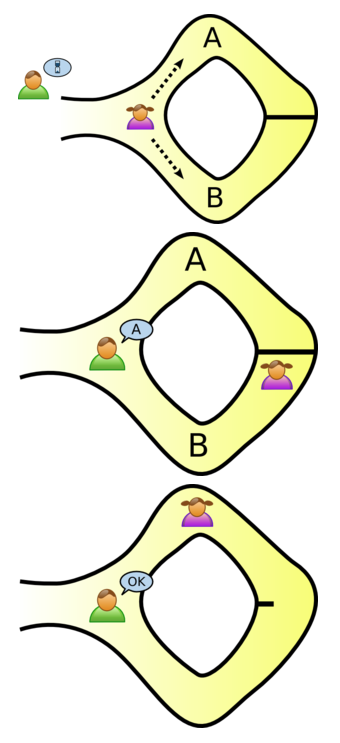
\includegraphics[scale = 0.5]{Images/Ali_Baba.png}%
\captionof{figure}{Ali Baba cave}
\label{fig:Ali Baba cave}
\columnbreak
This one is the Ali Baba cave example. The cave is ring-shaped and has a magic door (whose opening requires a secret key) at the opposite side of the entrance (Victor the verifier is aware of its presence). Peggy the prover enters the cave and randomly chooses a path (A or B) without being seen by Victor. Then Victor eventually enters and shouts the name of the path he wants Peggy to take when coming outside.
\end{multicols}
\noindent
Provided that Peggy effectively knows the secret key, she can simply open the door and exit where requested. On the other hand, if she doesn't know the secret key, her 50\% probability of guessing the right path at the first attempt would eventually vanish after several repetitions of the experiment. \\
Another common example is the graph 3-colorability problem, that the interested reader can find in \cite{PedroFranco}.\\
Eventually, we would like to present an example with higher cryptographic relevance. It turns out that a prover can possibly prove in zero-knowledge that he knows the discrete logarithm $q$ of a given value $c = g^q$, $g$ being the generator of the underlying cyclic group (according to notation in Appendix \ref{cyclic_groups}). There are many of such proofs; we present the Schnorr protocol (in its interactive form).
\begin{itemize}
    \item The prover selects a random number $r$, computes $g^r \mod{n}$ and sends it to the verifier.
    \item The verifier challenges the prover by sending to him a random value $e$. 
    \item The prover replies to the challenge computing $u = r + e\cdot q \mod{n} $ and sending it to the verifier.
    \item The verifier accepts if $g^u \mod{n} = g^r\cdot c^e \mod{n}$. Indeed, $g^u \mod{n} = g^{r + e\cdot q} \mod{n}$ = $g^r {(g^q)}^e \mod{n}$ = $g^r c^e \mod{n}$.
\end{itemize}
Once again, the proof is successfully carried out in zero-knowledge as the verifier can get no clue about $q$ and at the same time would unmask a cheating prover.\\ 
The provided examples are kinds of interactive proofs we are not strictly interested in\footnote{Indeed as we will see, the solution \textit{confidential transactions} adopt is non-interactive. Moreover, even in previous subsections we have always presented the primitives in their non-interactive form.}, but succeed in giving an impressive idea of how these proofs work. Their non-interactive counterparts (in which there's no interaction between prover and verifier) are obtained via the Fiat-Shamir heuristic, where the challenges by the verifier are replaced by the result of the hash of some intermediate result. 

\section{Ring signatures}
\label{ring_signatures}
Initially introduced in \cite{LeakSecret}, ring signatures are a cryptographic primitive allowing for any actor in a group to provide a digital signature\footnote{We are not interested in giving a formal definition of digital signature and we refer to \cite{UnderstandingCrypto}.} on behalf of the group itself, but preserving the anonymity of the signer (\textit{signer ambiguity}). More precisely, the actual signer can select any set of potential signers which includes himself (provided he knows a public key for each of them) and signs a message with his own private key in a way that the whole signature does not leak any information about who has effectively produced the signature. Moreover, the selected possible signers are usually not aware of the fact that their public key has been used in a ring signature scheme (like a multiparty 1-of-$m$ signature scheme without cooperation from the other $m-1$ members). Thus, it shouldn't be much of a surprise that one of the described application in \cite{LeakSecret} was whistleblowing, namely the possibility of leaking a disgraceful secret of a group of people (think as an example to an episode of corruption inside a city council) by one of the members of the group in a way that the whistleblower could not be identified, but at the same time with certainty that the leak came from a member of the group.\\
Given that, a ring signature scheme could be seen as a variant of a digital signature scheme in which the single verification (public) key is replaced by a ring of verification (public) keys and one private key only is required to produce a valid signature; moreover, given that the actual signer does not know the private keys corresponding to the public keys of the other group members, these are generally forged (but obviously indistinguishable to real ones).\\
A ring signature scheme involves two procedures: \begin{itemize}
    \item $ring-sign(m, Q_1, Q_2, \dots, Q_s, q_s)$: it produces a ring signature $\sigma$ for the message $m$ given the public keys $Q_1, Q_2, \dots, Q_s$ of the $s$ ring members, together with the private key $q_s$ of the $s^{th}$ member (the signer).
    \item $ring-verify(m,\sigma)$: it accepts a message $m$ and a signature $\sigma$ (including the pubkeys of all the possible signers) and outputs either true or false.
\end{itemize}
We are not going to present here the algorithm that underlies the construction of ring signatures in \cite{LeakSecret} both because it would require migrating to the RSA\footnote{\url{https://en.wikipedia.org/wiki/RSA_(cryptosystem)}} setting and because in the next section we will directly describe the version adopted by \textit{confidential transactions}. Before passing to the next primitive, we only summarize all of the features of ring-signature schemes. Other than being signer-ambiguous signature schemes (there is no possibility to revoke the anonymity of the signer and more precisely a verifier has a probability equal to $\frac{1}{s}$ to guess the identity of the real signer), they are setup-free signature schemes. This means that there is not a pre-arranged group of members (this is particularly relevant in the comparison with group signature schemes from which ring-signatures derive and whose underlying mechanism is basically the same apart from the presence of a trusted group manager who selects the ring members and can unmask the anonymity of misbehaving signers). In the end, it has to be noticed that the signature size grows linearly with the number of rings.

\section{Elliptic Curve Diffie-Hellman}
\label{ECDH}
The elliptic curve Diffie-Hellman primitive is a cryptographic primitive which is at the basis of the ECDH Key Exchange scheme.\\
In turn, the elliptic curve Diffie-Hellman Key Exchange (ECDH) is a key agreement scheme based on ECC, thus relying on the hardness of the ECDLP. It is the EC counterpart of the well known\footnote{In cryptography at least.} Diffie-Hellman Key Exchange (DHKE) protocol. In this section we just present the scheme for the elliptic curve version.\\
It allows two entities, both endowed with an elliptic curve private-public key pair, to engage in a key agreement scheme and establish a shared secret over an insecure (yet authenticated) channel. The shared secret can then be both used directly as key or as seed to derive other key(s), for instance (but it is just a possibility) via a deterministic generation procedure like RFC6979 (see \cite{rfc6979}).
\subsection{ECDH primitive}
The primitive is built in such a way that both the parties by means of one of their own private key and one of the public key of the other party can recover, autonomously, the same (shared) secret.\\
Here how's the primitive built. Suppose Alice and Bob want to establish a shared secret. The primitive is run autonomously by both and takes as input valid elliptic curve domain parameters $T$\footnote{$T$ = $(p, a, b, G, n, h)$; $p$ specifies the prime finite field $\mathbb{F}_p$; $a,b \in \mathbb{F}_p$ are the coefficients of the elliptic curve equation; $G \in E(\mathbb{F}_p)$ is the elliptic curve generator point; $n$ is the order of $G$, that coincides with the number of points of the cyclic subgroup generated by $G$; $h = \#E(\mathbb{F}_p)/\ n$ is the so called cofactor.}, a private key owned by who is running the procedure ($q_A$ for Alice, $q_B$ for Bob) and the public key corresponding to the other party private key (Alice takes $Q_B$=$q_BG$ as input, Bob takes $Q_A$=$q_AG$ as input\footnote{Though, Alice does not obviously know $q_B$, nor Bob $q_A$.}). The output is a shared secret field element $z$ or the string ``invalid" otherwise.\\
The algorithm below refers to the generation of the shared secret from Alice. The same can be done for Bob, by carefully exchanging the roles of the parameters.
\begin{algorithm}
	\caption{ECDH primitive}
	\label{alg:ECDH}
	\begin{algorithmic}[1]
		\Procedure{ecdh}{$T, \ q_A, \ Q_B$}
		\State $S = (x_S,y_S) \gets q_AQ_B$
		\State assert $S \neq \{\infty\}$
		\If {$S = \{\infty\}$}
		\State \textbf{return} ``invalid"
		\EndIf 
		\State \textbf{return} $z \gets x_S \mod{n}$ 
		\EndProcedure
	\end{algorithmic}
\end{algorithm}\\
It turns out to be straightforward to prove that the shared secret computed by both parties is the same. Alice: $q_AQ_B = q_A(q_BG)$; Bob: $q_BQ_A = q_B(q_AG)$ $\rightarrow$ by associativity of the group operation (point addition), the result holds and both compute $S=q_Aq_BG$.
\subsection{ECDH Key Exchange protocol}
According to notation in \cite{Sec}, the key exchange protocol involves a \textit{setup} phase, a \textit{key deployment} procedure and a \textit{key agreement} operation (which actually exploits the ECDH primitive).
Here's a simple graphical representation of the key exchange protocol combining the key deployment phase (in its associated public keys exchange phase) and an instance of the ECDH primitive explained above.
\begin{center}
	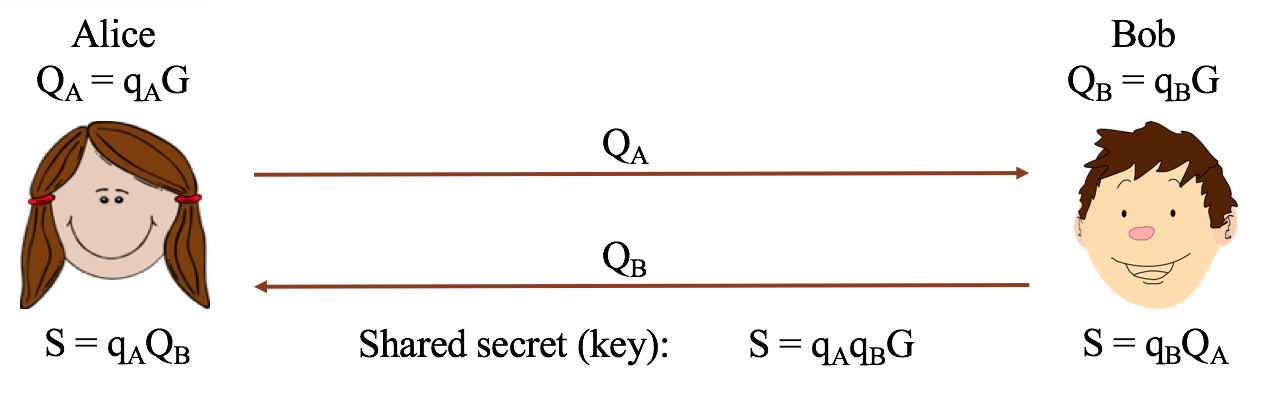
\includegraphics[scale = 0.55]{Images/ECDH.png}
	\captionof{figure}{ECDH key exchange}
	\label{fig:ECDH}
\end{center}
The \textit{setup} phase defines the choice of the elliptic curve domain parameters.\\
The \textit{key deployment} phase requires both parties establishing valid private-public key pairs $(q_A,Q_A)$, $(q_B,Q_B)$ and exchanging their public keys $Q_A$ and $Q_B$ (with further assurance of the public keys being valid ones).\\
The \textit{key agreement} operation defines a way to obtain shared keying data from a shared secret by means of a suitable key derivation function. Observe, however, that the keying data might not directly be used as a key, this just depends on the application.\\ The algorithm below refers to the generation of the shared key by Alice. Bob's algorithm is straightforward and just requires rearrangement of the parameters. We first describe the key derivation function (KDF), taking as inputs an octet\footnote{To keep it simple we can consider an octet being equivalent to a byte.} string $Z$ derived from the field element $z \in \mathbb{F}_n$ outputted by the ECDH primitive,\footnote{For more details on the \textit{field-to-octet} conversion, see \cite{Sec}.} the integers \textit{keydatalen}, \textit{hashlen}, \textit{hashmaxlen} which refer to the length in octets respectively of shared key, hash values and maximum lenght of messages that can be hashed with the given hash function. It outputs a shared key $K$ (octet string) or ``invalid". 
\begin{algorithm}
	\caption{Key Derivation Function}
	\label{alg:KDF}
	\begin{algorithmic}[1]
		\Procedure{kdf}{$Z, \ keydatalen, \ hashlen, \ hashmaxlen $}
		\State assert $|Z| + 4 < hashmaxlen $, ``invalid"
		\State assert $keydatalen < hashmaxlen * (2^{32} -1) $, ``invalid"
		\State $count \gets 1 $  \Comment{4 octet, big-endian string}
		\For {$i\gets 1, \lceil{keydatalen /\ hashlen}\rceil$}
		\State $K_i \gets hash(Z||count)$
		\State $count \gets count + 1$
		\State $i \gets i + 1$
		\EndFor
		\State $K \gets K \verb|>>=| (keydatalen - hashlen)$ \Comment{leftmost keydatalen octects of $K_1||\dots||K_{\lceil{keydatalen /\ hashlen}\rceil}$}
		\State \textbf{return} $K$ 
		\EndProcedure
	\end{algorithmic}
\end{algorithm}\\
Thus, the whole key agreement operation requires deriving a shared field element $z \in \mathbb{F}_n$ by running an instance of the ECDH primitive, converting it to an octet string to give as input to the KDF and consequently deriving a shared key.\\
For what concerns security arguments, it is required the ECDHP (elliptic curve Diffie-Hellman problem) to be hard to solve. It comes out it is closely related to the ECDLP, a third party willing to break it has to solve either $q_A = \log_G{Q_A}$ or $q_B = \log_G{Q_B}$. Consequently, provided a care choice of the parameters during the setup phase, the more powerful algorithms to break it are basically the same presented above for the ECDLP ($\sim O(|\mathbb{G}|^{\frac{1}{2}})$ steps). What that means practically is that with an elliptic curve group order higher than $2^{160}$ (i.e. $160$ bits)\footnote{Bearing in mind that, as a rule of thumb, security levels of more than 80 bits can be considered satisfactory.} the ECDHP wouldn't be possibly broken.\\ 
Then, another important security assumption relies on the so-called channel authentication for public key exchange, required to prevent \textit{man-in-the-middle} attacks. The latter consist in an adversary eavesdropping over the channel and substituting Alice and Bob's public keys with his own public keys. If the channel is not authenticated,\footnote{Where authentication means that the recipient has strong reasons to believe that the communication is in place with the ``designated" sender and can be achieved by means of some protocols we do not present here.} this would prevent Alice and Bob being aware of sharing a secret with the eavesdropper rather than themselves.